\chapter{Measurement of differential single-top-quark cross sections at 13~TeV}
\label{ch:diff13}

\intro{A first measurement of normalized differential single-top-quark cross sections in $t$~channel as a function of the top quark transverse momentum and rapidity at 13~\TeV is presented. \Acrlong{pp} collision data corresponding to an integrated luminosity of 2.3~\invfb are analyzed which were recorded in 2015 with the \gls{cms} experiment. Events containing one isolated muon and two or three jets are selected and a \acrlong{bdt} is trained for separating signal from background events further. The amount of signal events as a function of the top quark transverse momentum and rapidity is estimated by multiple fits. The results are unfolded to parton level and compared to predictions by various \acrlong{mc} generators. No significant deviations are observed. The measurement has been published in Ref.~\cite{CMS-PAS-TOP-16-004}.
}

%##############################################
\section{Analysis strategy}
%##############################################

The strategy to measure normalized differential single-top-quark cross sections in $t$~channel as a function of the top quark \pt and rapidity is as follows. Events containing one isolated muon and two or three jets are selected. Then, a \gls{bdt} is trained to obtain a powerful discriminant for separating signal from background events. An extended \gls{ml} fit is setup to estimate the amount of signal and background events in data. The distributions of the transverse W~boson mass and the \gls{bdt} discriminant are fitted simultaneously in the signal and two \ttbar control regions. During the fit, the contamination by multijet events is also estimated using a data-driven model of its shape from a sideband region for which the muon isolation during the event selection is inverted. Multiple fits are performed in intervals of the top quark transverse momentum and rapidity. The differential cross sections are inferred by passing the fit results directly to the unfolding. The impact through source of systematic uncertainties on the differential cross section shape is evaluated by repeating the measurement with modified templates.

\todo{check here}
This chosen strategy has multiple benefits. First, it does not require to define a signal-enriched region where the remaining backgrounds are subtracted from data prior to unfolding. Instead, the signal yields in intervals of the top quark \pt and rapidity are taken from the fits directly. Secondly, since no signal-enriched region is defined its selection does not need to found through an optimization procedure. No explicit selection to reject multijet events or on the \gls{bdt} discriminant is necessary to carry out the measurement. Only for validation purposes, events with $\mtw>50~\GeV$ are selected to verify the modeling of background processes in a multijet-depleted region. Lastly, residual differences in the estimated backgrounds yields between unfolding bins are profiled which reduces the impact by potential shortcomings in their modeling or a bias occurring through correlations of \gls{bdt} input observables with the top quark \pt and rapidity.

The measured normalized cross sections are compared to the predictions by various event generators.

%##############################################
\section{Event selection and simulated samples}
%##############################################

The measurement is based on \gls{pp} collision events corresponding to 2.3~\invfb which were recorded by the \gls{cms} experiment in 2015 at a \acrlong{cm} energy of 13~\TeV. An isolated muon trigger is employed for recording data events which requires the presence of an isolated muon candidate with a transverse momentum of at least $20~\GeV$ within $|\eta|<2.4$. In the analysis, the muon candidate has to have a momentum of $\pt>22$ within $|\eta|<2.4$ and pass tight identification requirements. A relative \gls{deltabeta}-based isolation of $\muiso<6\%$, calculated from the transverse energy deposits of charged and neutral hadrons, photons, and tracks associated to pileup within a cone of $\Delta R<0.4$, is required. The isolation is explicitly chosen tighter here compared to corresponding analyses at 8~\TeV (e.g. Ch.~\ref{ch:polarization}) in which $\muiso<12\%$ was required instead. The distribution of the relative muon isolation after applying the complete events selection with the exception of the isolation is presented in Fig.~\ref{fig:diff13-reliso}. Here, the multijet template is taken exceptionally from simulation and scaled such that it fits to the bulk of the distribution. The deviation at high isolation values can be attributed to the trigger emulation in simulation which has a somewhat different compared to data. The distribution motivate a tighter isolation here to counter observed the larger contamination by multijet events at 13~\TeV.

\myfigure{\label{fig:diff13-reliso} Distribution of the relative \gls{deltabeta}-based muon isolation in 2j1t. The multijet template is taken from simulation.}{
\subfloat[]{\adjincludegraphics[height=4.8cm,trim={0 0 {0.\width} 0},clip]{figures/differential/plots/2j1t/2j1t_relIso_qcdnone.pdf}}
}

\Gls{pf} candidates are clustered into jets using the anti-\kt algorithm with a distance parameter of $R=0.4$. The influence by pileup is mitigated through the \gls{chs} technique~\cite{CMS-PAS-JME-14-001}. 



 

\myfigure{\label{fig:diff13-topmass} Distributions of the reconstructed top quark mass in signal and control regions.}{
\subfloat[]{\adjincludegraphics[height=4.8cm,trim={0 0 {0.16\width} 0},clip]{figures/differential/plots/2j0t/2j0t_top_mass_qcdnone_nol.pdf}}
\subfloat[]{\adjincludegraphics[height=4.8cm,trim={0 0 {0.\width} 0},clip]{figures/differential/plots/2j1t/2j1t_top_mass_qcdnone.pdf}}\\
\subfloat[]{\adjincludegraphics[height=4.8cm,trim={0 0 {0.16\width} 0},clip]{figures/differential/plots/3j1t/3j1t_top_mass_qcdnone_nol.pdf}}
\subfloat[]{\adjincludegraphics[height=4.8cm,trim={0 0 {0.\width} 0},clip]{figures/differential/plots/3j2t/3j2t_top_mass_qcdnone.pdf}}
}


%##############################################
\section{Modeling}
%##############################################
\label{sec:diff13-modeling}
Njets, Nbjets
show cosTheta in 2j0t for wjet modeling for amc and mg samples if possible


%##############################################
\section{BDT training}
%##############################################
\label{sec:diff13-bdt}

%##############################################
\section{Signal extraction}
%##############################################


%##############################################
\section{Unfolding}
%##############################################

%##############################################
\section{Results}
%##############################################


%##############################################
\section{Prospects}
%##############################################

%##############################################
\subsection{Extended samples}
%##############################################

%##############################################
\subsection{Fiducial studies}
%##############################################
\label{sec:diff13-fiducial-studies}



Figures~\ref{fig:technique-particle-level-muonpt} and~\ref{fig:technique-particle-level-muoneta} show a comparison of the muon $\pt$ and pseudorapidity at reconstruction, particle, and parton level after selecting events with one muon at each level respectively. The top panels demonstrate a high overlap of the events selected at reconstruction level with the ones at particle and parton level. The acceptance rises with the muon momentum from about 40\% to 90\% due to the relative isolation requirement for reconstructed muons. The number of jets is presented in Fig.~\ref{fig:technique-particle-level-njet}. Due to the jet energy scale correction, 


dressed leptons (cone algorithms associates photons to leptons but does not cluster close leptons), tau decays, jet clustering (no neutrinos/leptons), b-tagging,




particle level overlap: tightMu: >99\%, 2jets: 80\%, 2j1t: 70\%


\myfigure[p]{\label{fig:technique-particle-level}Comparison of expected event densities for $1~\invfb$ at $13~\TeV$ after applying the event selection at reconstruction, particle, and parton level respectively:  (a)~muon $\pt$, (b)~muon rapidity, and (c)~number of jets after requiring one isolated and tight muon; (d)~number of b-tagged jets, (e)~$\pt$ and (f)~pseudorapidity of the spectator jet after requiring one isolated, tight muon and two jets where in (e,f) one jet is additionally required to be b-tagged at reconstruction level. Top panels show the common events selected at reconstruction level while the bottom panels display the acceptance.}{
\subfloat[\label{fig:technique-particle-level-muonpt}]{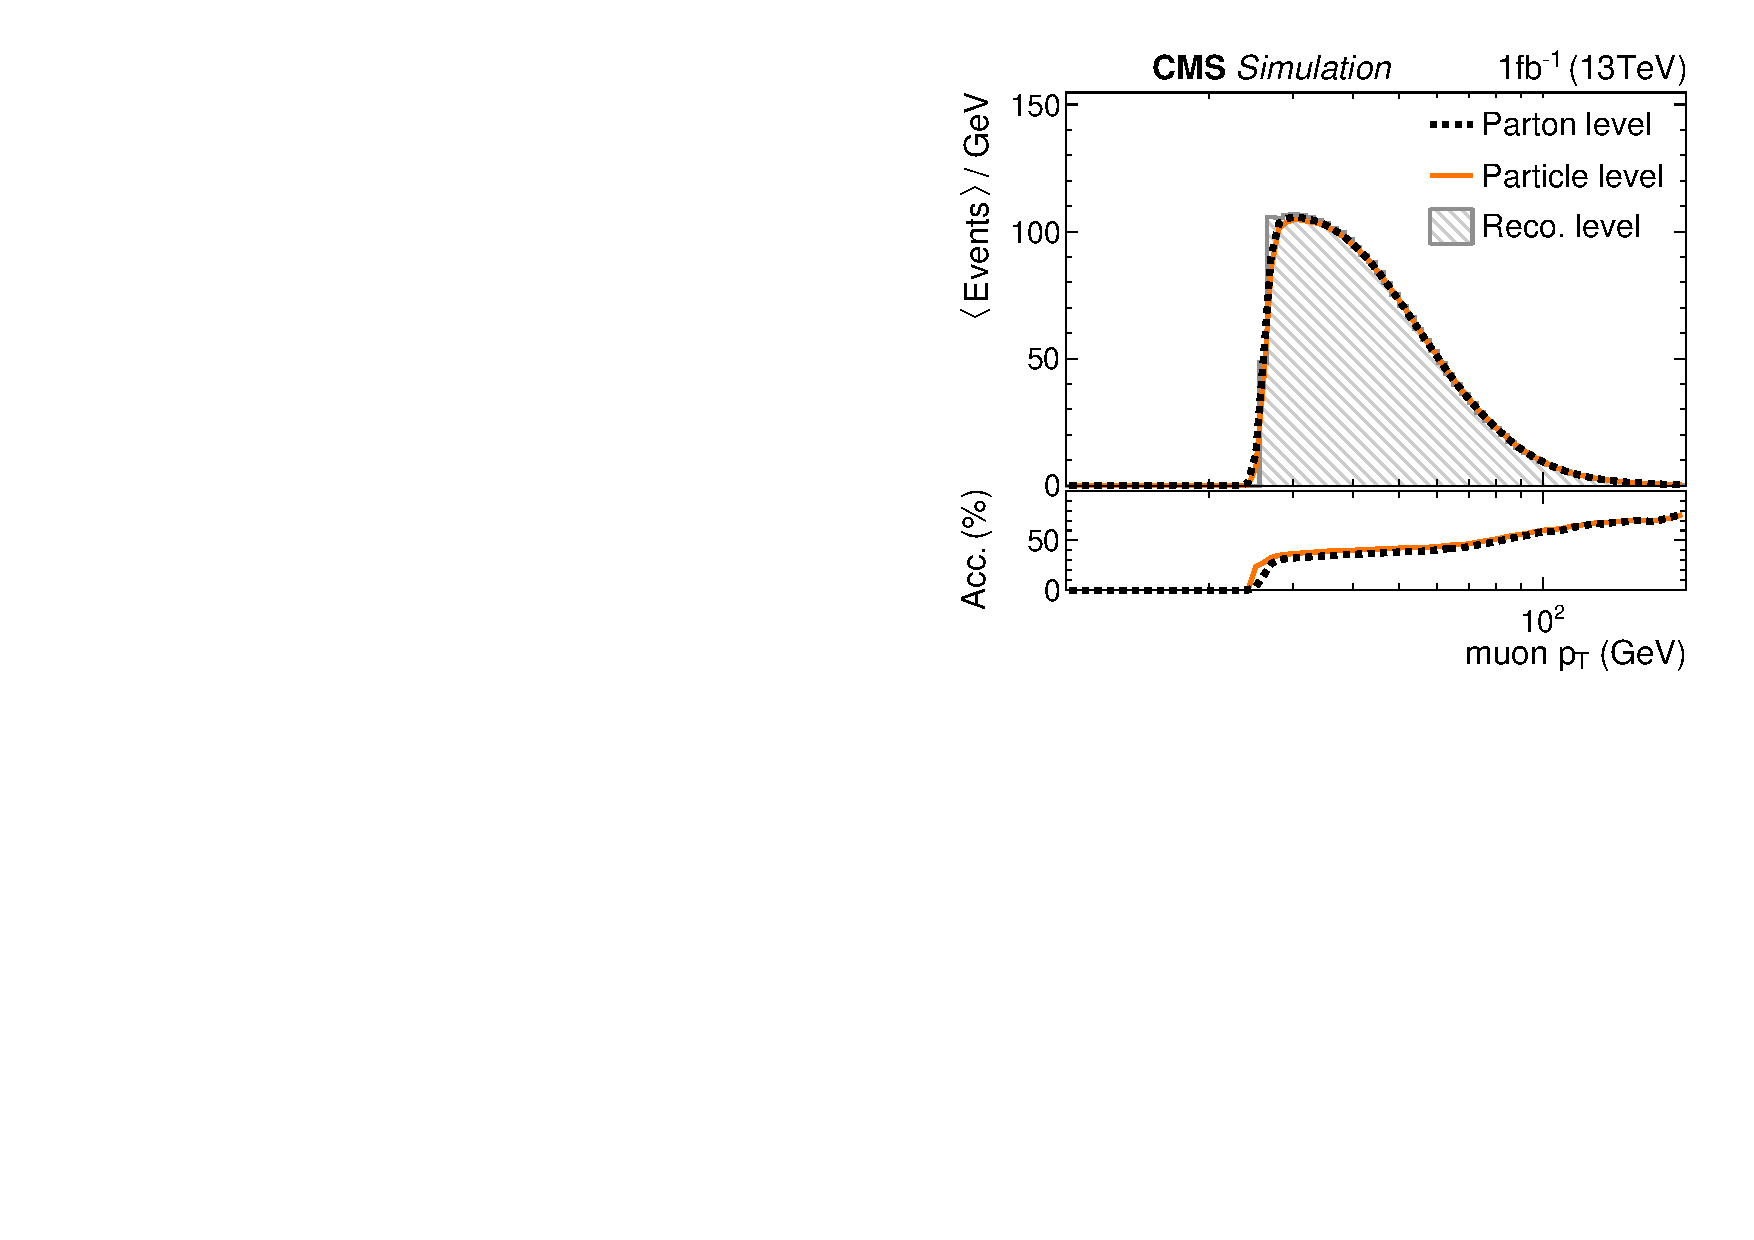
\includegraphics[width=0.48\textwidth]{figures/technique/muon_particle_logpt.pdf}}\hspace{0.03\textwidth}
\subfloat[\label{fig:technique-particle-level-muoneta}]{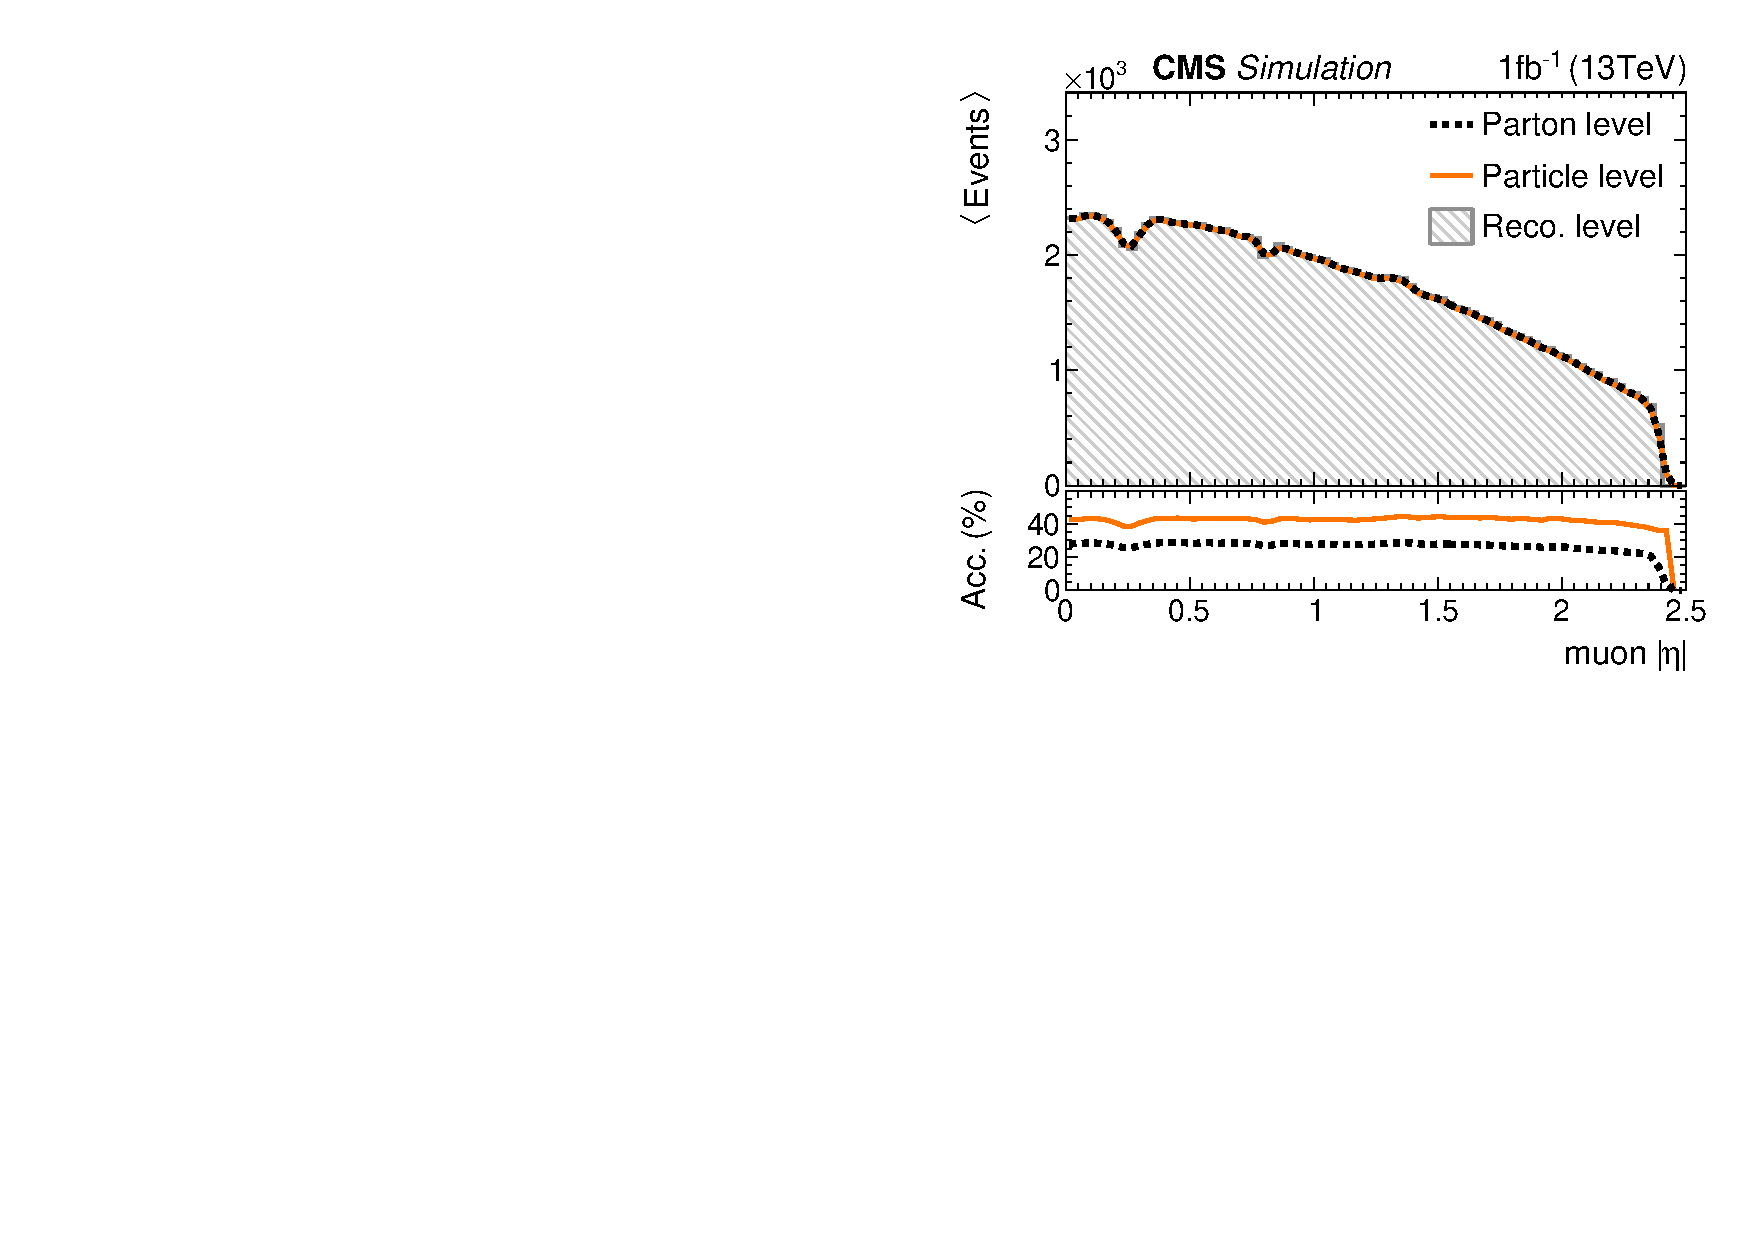
\includegraphics[width=0.48\textwidth]{figures/technique/muon_particle_abseta.pdf}}\\
\subfloat[\label{fig:technique-particle-level-njet}]{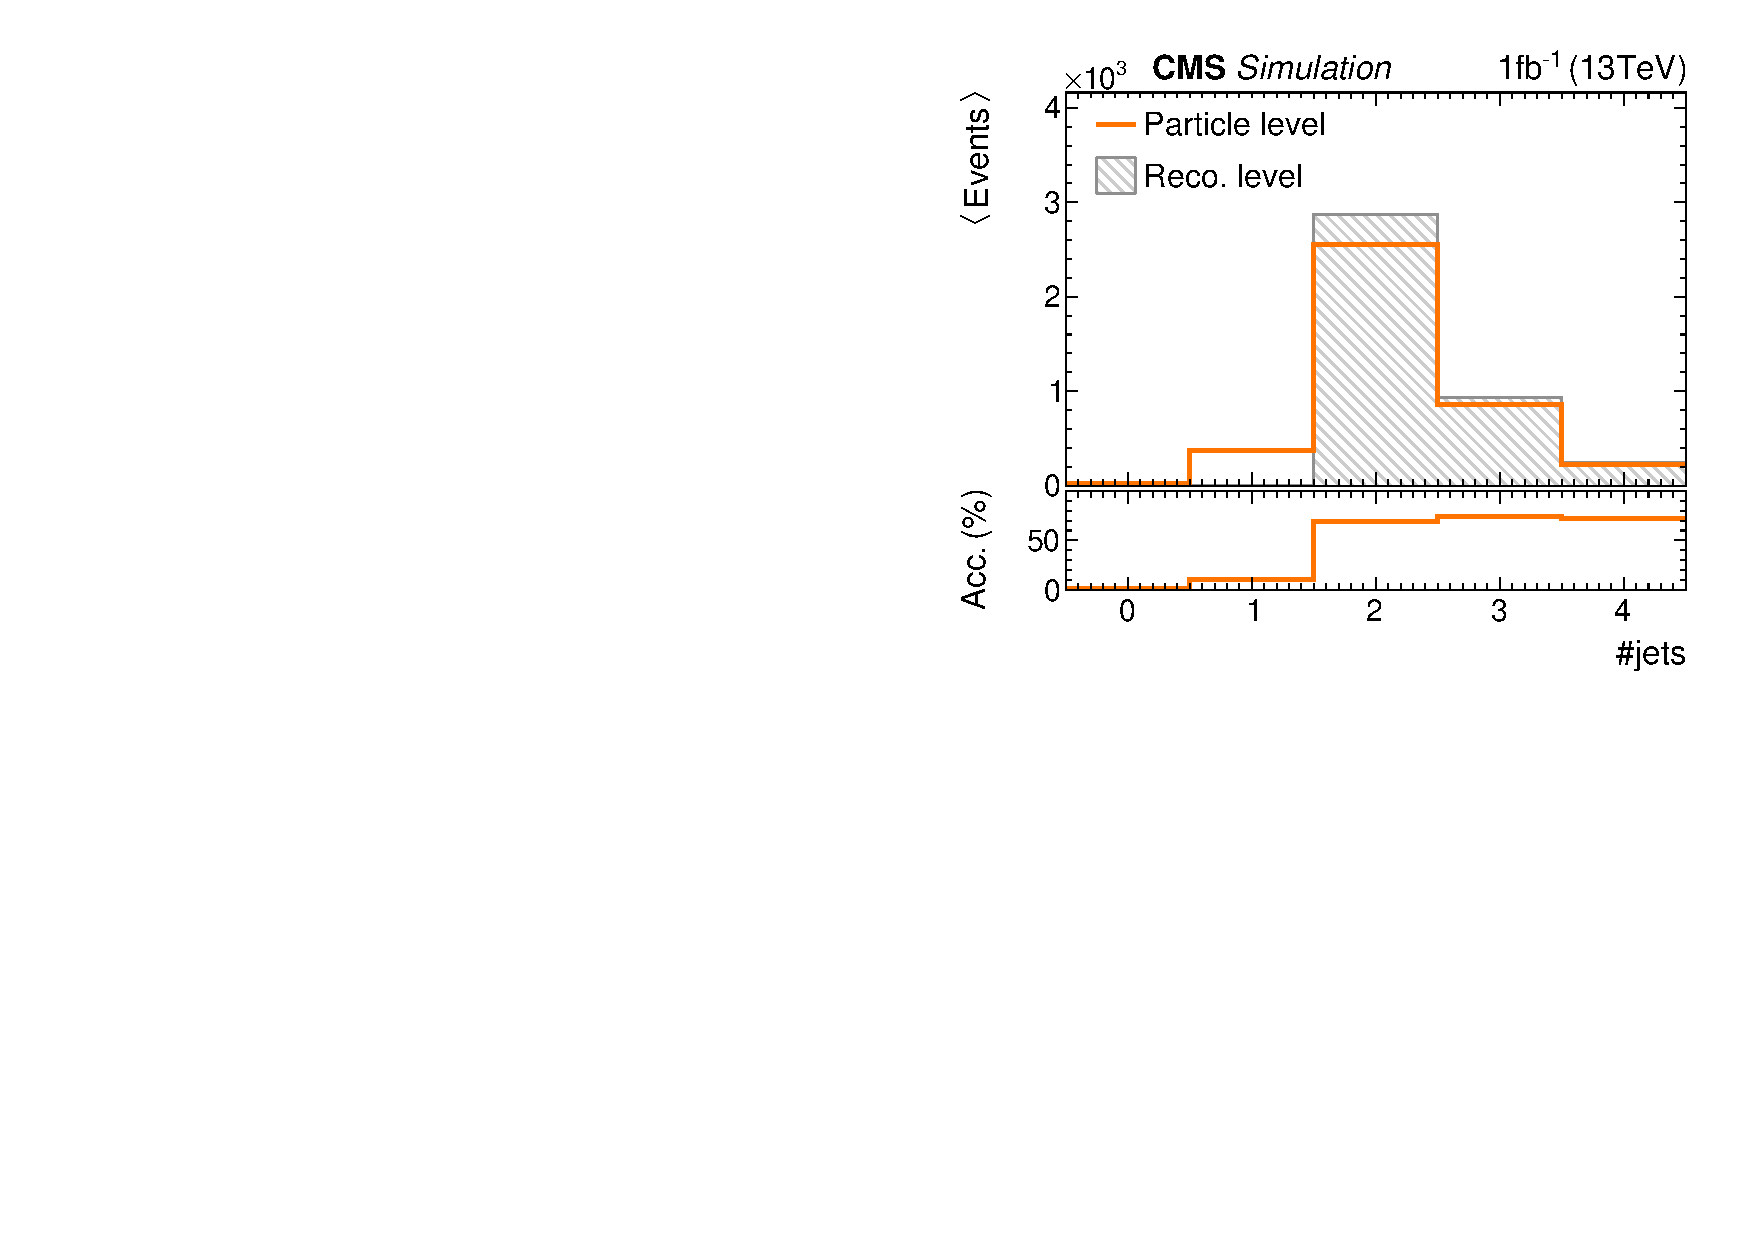
\includegraphics[width=0.48\textwidth]{figures/technique/njet_particle.pdf}}\hspace{0.03\textwidth}
\subfloat[\label{fig:technique-particle-level-nbjet}]{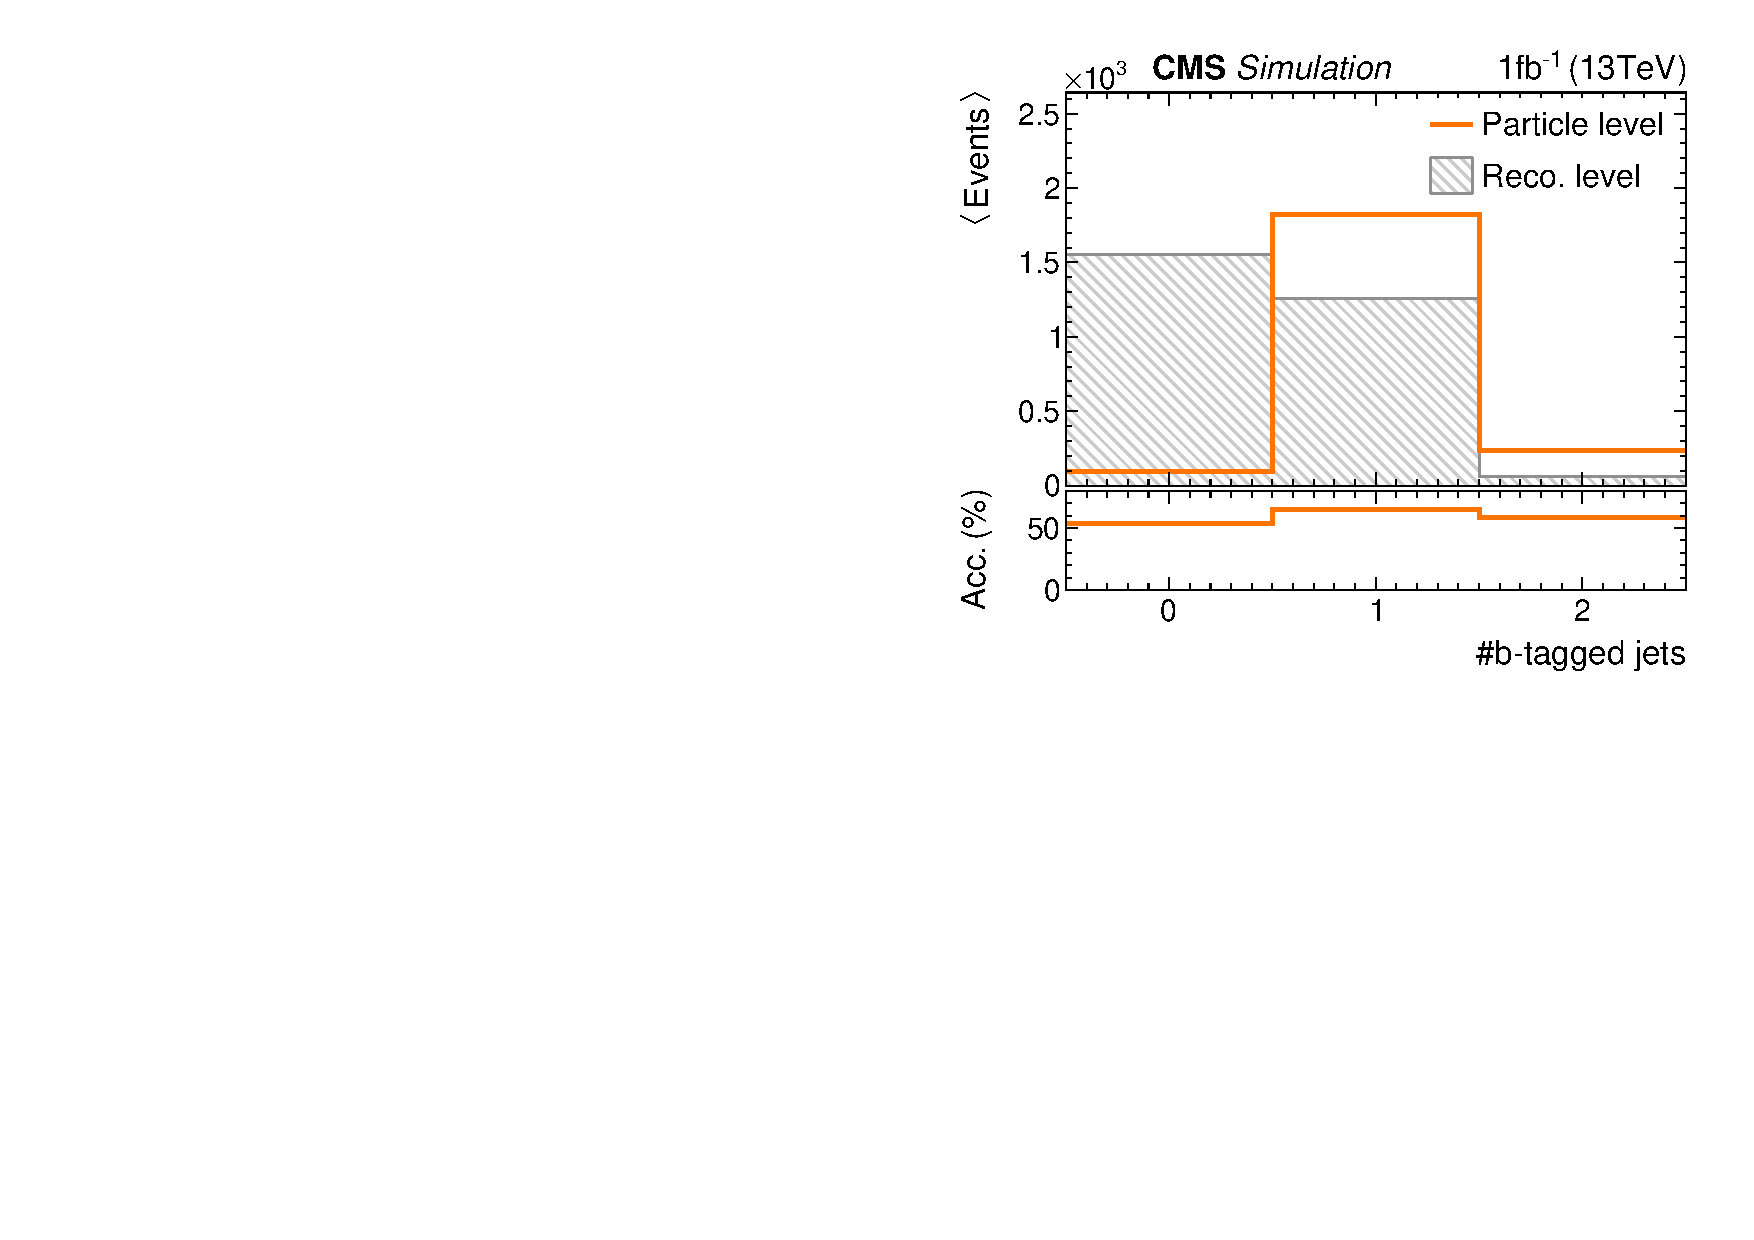
\includegraphics[width=0.48\textwidth]{figures/technique/nbjet_particle.pdf}}\\
\subfloat[\label{fig:technique-particle-level-ljetpt}]{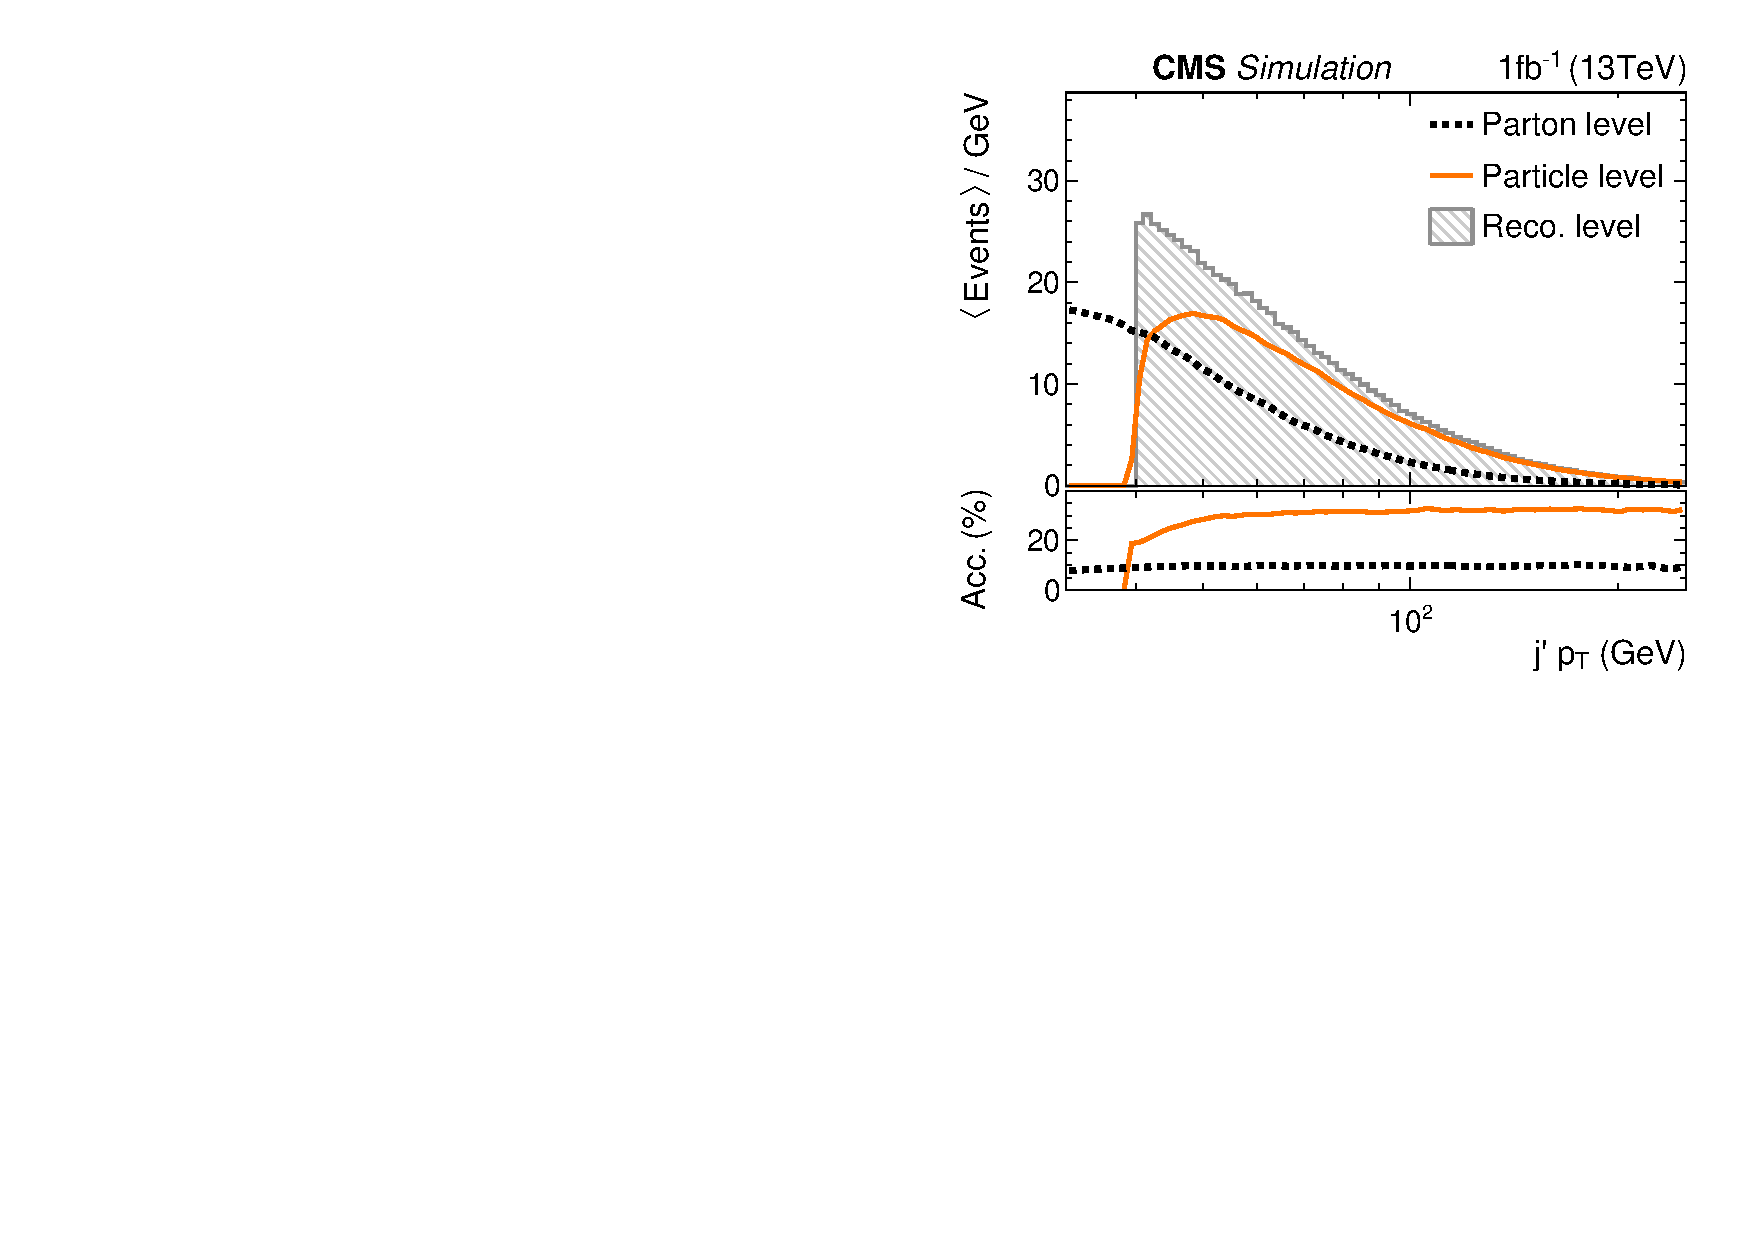
\includegraphics[width=0.48\textwidth]{figures/technique/ljet_particle_logpt.pdf}}\hspace{0.03\textwidth}
\subfloat[\label{fig:technique-particle-level-ljeteta}]{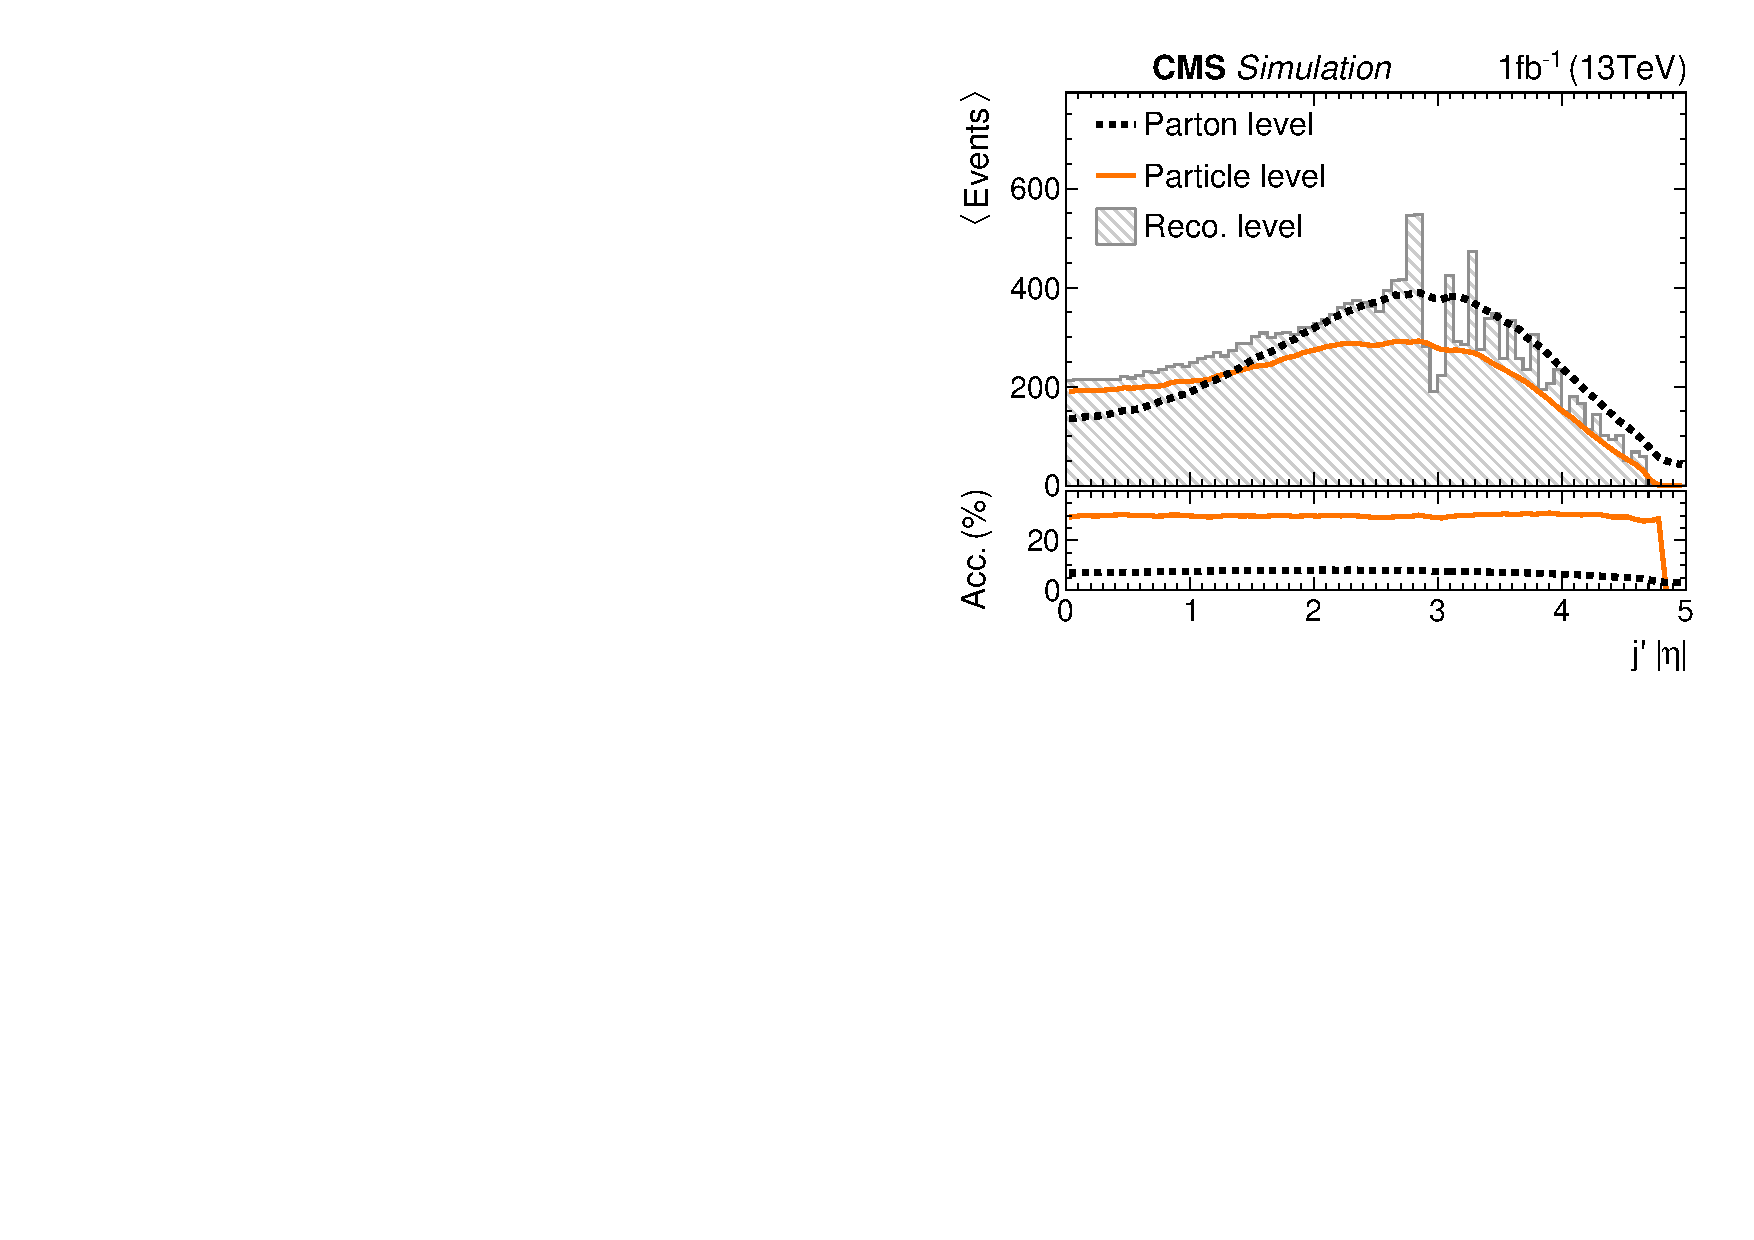
\includegraphics[width=0.48\textwidth]{figures/technique/ljet_particle_eta.pdf}}
}

\myfigure[phtb]{\label{fig:technique-particle-top}Comparison of event selection at reconstruction and particle level.}{
\subfloat[]{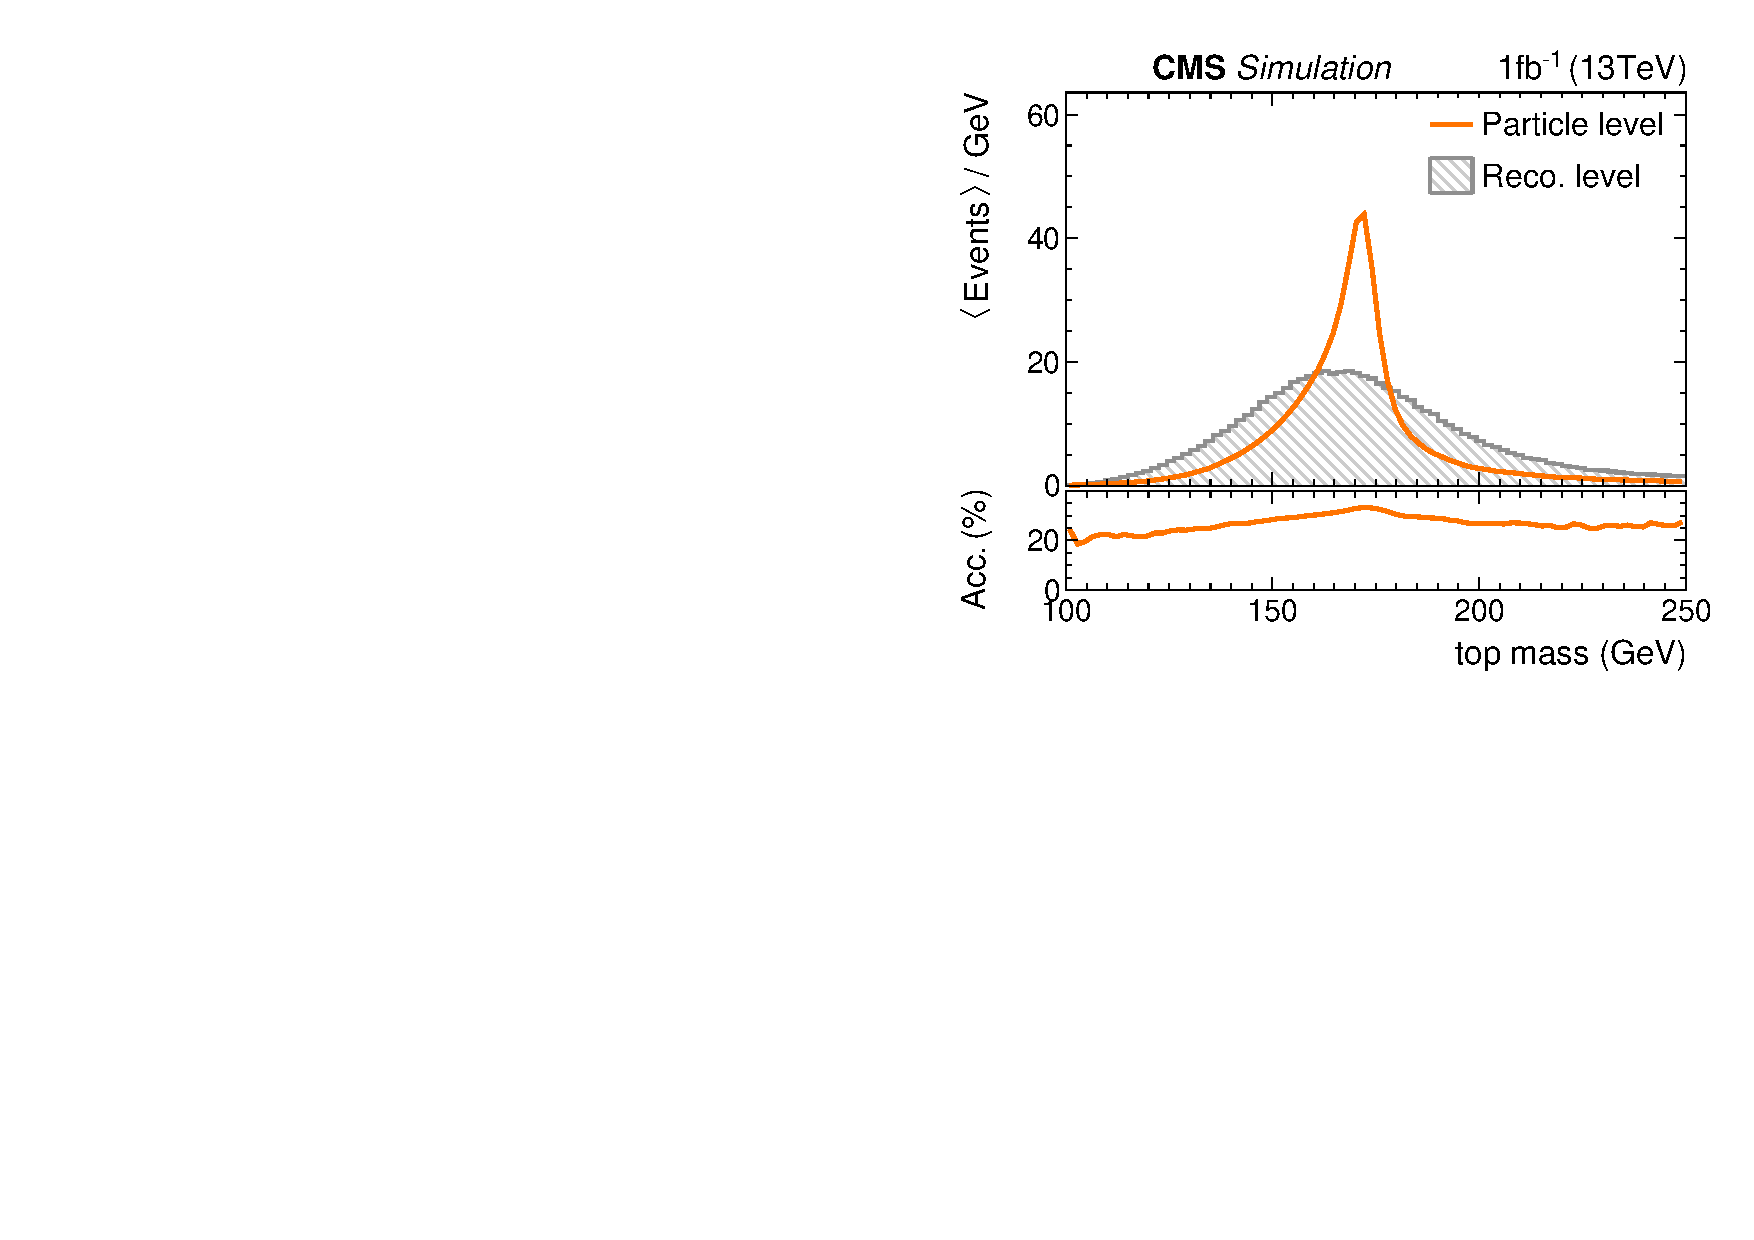
\includegraphics[width=0.48\textwidth]{figures/technique/top_particle_mass.pdf}}\hspace{0.03\textwidth}
\subfloat[]{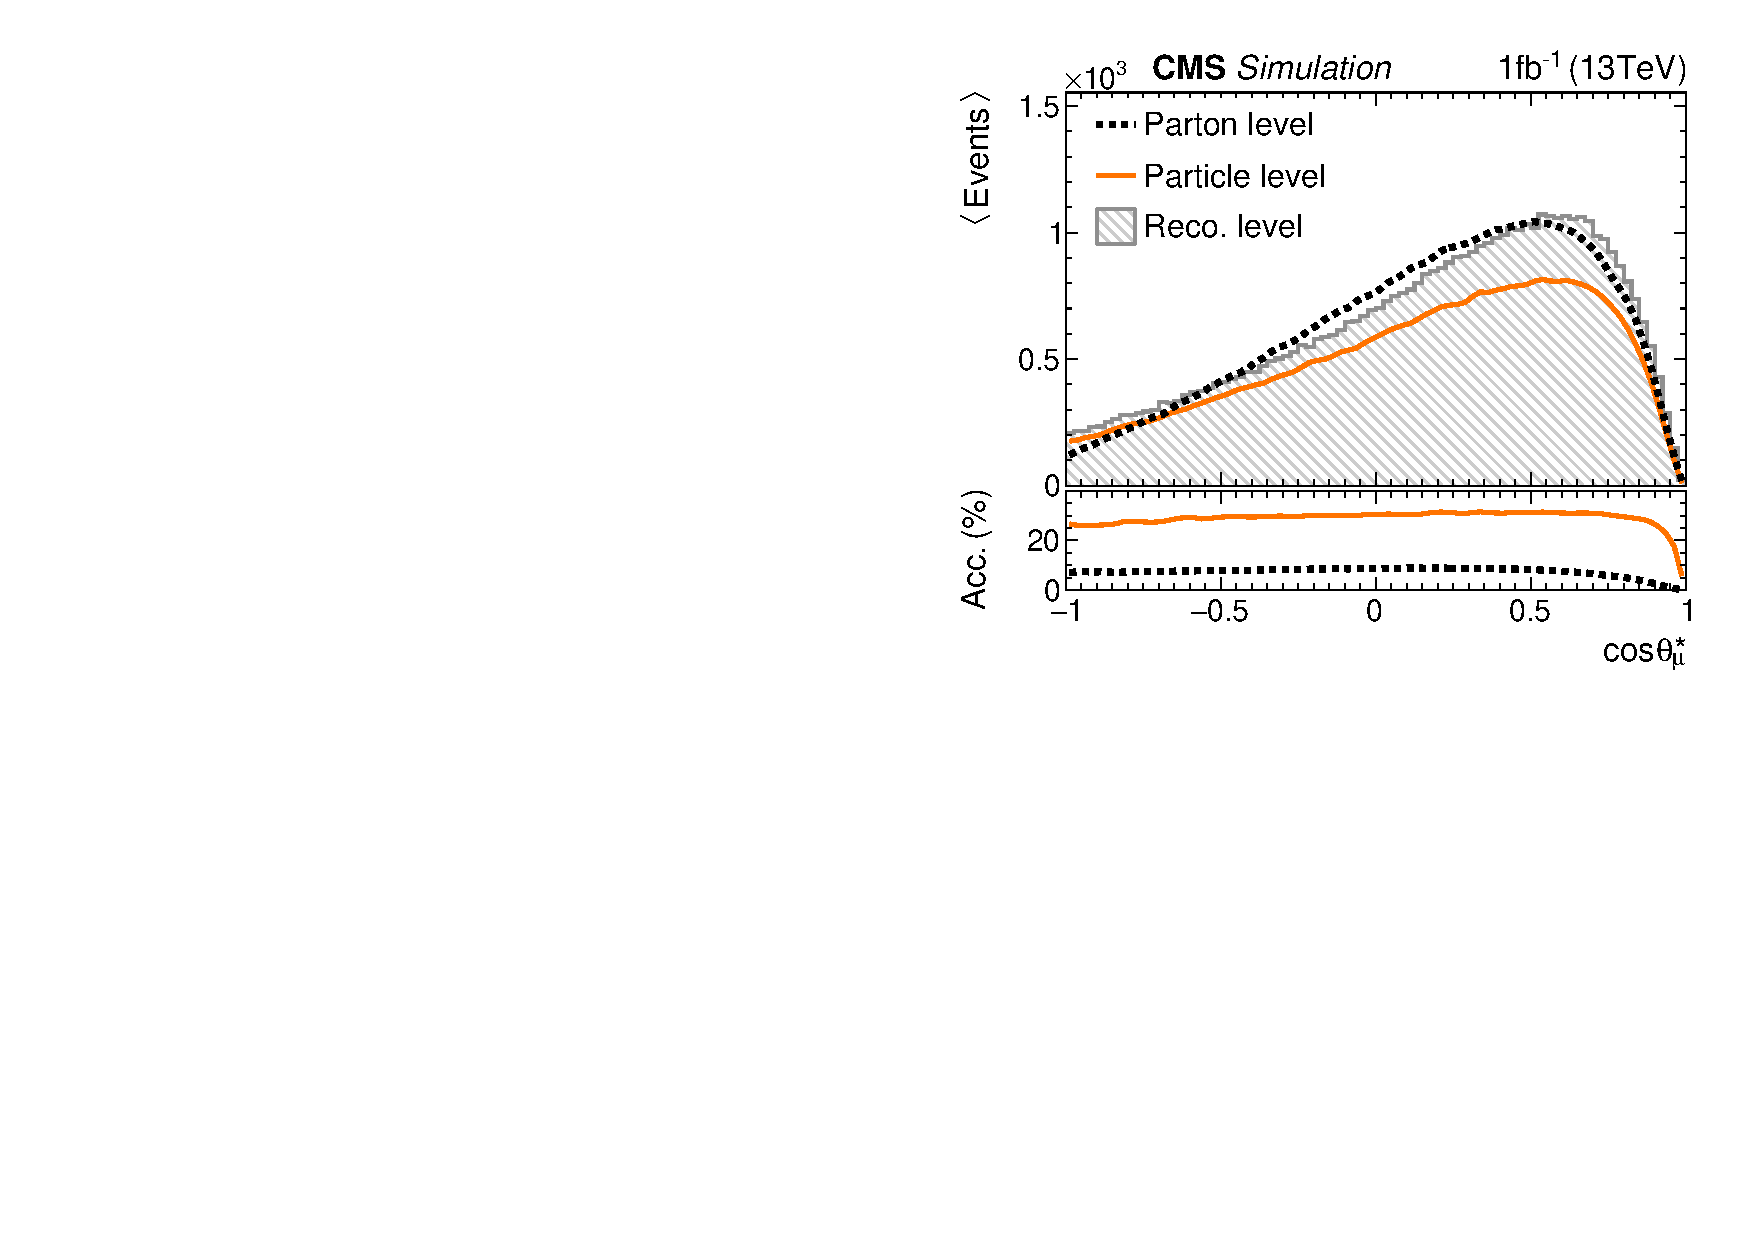
\includegraphics[width=0.48\textwidth]{figures/technique/cosTheta_particle.pdf}}
}
